\documentclass{article}
\usepackage[utf8]{inputenc}
\usepackage{amsmath}
\usepackage{graphicx}
\graphicspath{ {images/} }

\begin{document}
\begin{equation*}
Ç : \begin{bmatrix}
 p & q 
\end{bmatrix} \cup 
\begin{bmatrix}
q & p 
\end{bmatrix}\cup  (p \quad q)
\end{equation*}
olarak yazabiliriz.
\\ \\
Düğümlere ilişkin bu açıklamadan sonra $Y_{ab}$ ve $Y_{cd}$ yollarının uçdüğümlerinin bağıl konumlarına göre ortaya çıkan değişik durumların incelenmesine
geçelim.
\\ \\ 
\textit{Durum 1:}
\begin{equation*}
c \in  [a,u]
\quad \quad 
ve \quad \quad d \in  [b,v] \quad
(Şekil \quad4.2.2a)
\end{equation*}
\\ \\ 
ya da 
\begin{equation*}
c \in  [v,a]
\quad \quad 
ve \quad \quad d \in  [u,b] \quad
(Şekil\quad 4.2.2b)
\end{equation*}
\\
olduğunu düşünelim.
\\ \\
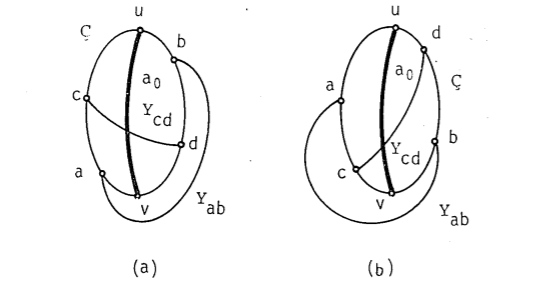
\includegraphics{sekil}\\\\

şekil 4.2.2 Durum 1 in incelemesi.

\end{document} 



